\chapter{Object Reconstruction}
\label{chap:reconstruction}

\section{Introduction}
\label{reco:sec:intro}

This chapter deals with the way in which the simulation and the data collected at the \CMS experiment are reconstructed and interpreted as particles for use in the \Hgg analysis. The reconstruction is done using custom software: elements of the reconstruction which are common to most analyses are performed using the \CMSSW package; further reconstruction elements which are specific to \Hgg are obtained using the \FLASHgg software. The \CMSSW software uses the \PF algorithm, in which energy deposits from the calorimeters and tracks from the tracker and muon system are combined to reconstruct individual particles which are likely to have passed through the detector. This algorithm is described in \Sec~\ref{reco:sec:pf}. The reconstruction and identification of particles often uses \MVA techniques, known as \BDT\s, which are described in \Sec~\ref{reco:sec:bdt}. 

The same reconstruction algorithms are applied both to actual data collected at the \CMS experiment, and to simulated samples where the interaction of generated particles with the \CMS sub-detectors is simulated. The way in which both data and simulation are obtained are described in \Sec~\ref{th:sec:samples}.

The work presented in this thesis involves the study of the Higgs boson decaying to photons, \Hgg. It has already been noted in \Sec~\ref{th:sec:higgs_decays} that \Hgg is one of the most sensitive ways in which the Higgs boson can be observed and its properties measured in the \LHC environment, and at \CMS in particular, despite having a small branching fraction ($\sim 0.2\% $) and an irreducible \SM background of \QCD processes which have two photons in the final state. The channel has the benefit of having a fully reconstructible final state and a clean signature. The experimental method to study the Higgs boson is therefore to look for a resonant Higgs boson peak on top of a continuous diphoton invariant mass spectrum.


The decay of the Higgs boson to photons, via a virtual loop of particles, can be treated as a two-body decay. It is easy to show that the invariant mass of the diphoton system (\mgg), i.e. the invariant mass of the Higgs boson, is given by:
\begin{equation}
\label{reco:eq:mgg}
 \mgg = \sqrt{2 E_{\gamma}^1 E_{\gamma}^2 (1-\cos\alpha)}, 
\end{equation}

where $E_{\gamma}^{1,2}$ represent the energies of the two photons and $\alpha$ represents the opening angle between them. The opening angle relies on identifying the spatial location of the Higgs boson decay. The method by which this is done is described in \Sec~\ref{th:sec:vertex}. Photons are reconstructed from deposits in the \CMS \ECAL. The methods with  which they are obtained and their energies are determined are described in \Sec~\ref{th:sec:photons}.

Higgs bosons are produced at the \LHC chiefly by the mechanisms described in \Sec~\ref{sec:th:higgs_production_modes}. In the dominant production mode, \ggH, at leading order the final state of interest consists only of the two decay photons. However, for other production modes, the Higgs boson can be produced in association with other particles. These additional objects in the detector can be reconstructed and provide information on the mode in which the Higgs boson was likely to have been produced. The methods used to reconstruct such additional objects are described in \Sec~\ref{reco:sec:other}.

\section{Reconstruction Tools}

\subsection{Particle-flow}
\label{reco:sec:pf}

The \PF event reconstruction algorithm (~\cite{CMS-PAS-PFT-09-001,CMS-PAS-PFT-10-001}) combines information from various \CMS \subdetector\s to reconstruct and identify individual particles. The inputs to this algorithm are the tracks reconstructed in the tracker and muon system, and the clusters of energy deposits in the \ECAL and \HCAL. The outputs of the algorithm are objects corresponding to stable particles (photons, electrons, muons, charged hadrons or neutral hadrons). In this scheme, \ECAL \SC\s which are not on the extrapolated trajectory of tracks from either the muon system or the tracker are identified as photons. Conversely, if a charged particle track in the tracker is associated to one or more \ECAL \SC (corresponding to the main electron and photons radiated by bremmstrahlung), then it can be identified as an electron. If a track in the tracker consistent with a track or multiple hits in the muon system, then it is identified as a muon. Tracks in the tracker which are not associated with any track in the muon system or any deposit in the \ECAL are interpreted as charged hadrons. Finally, deposits in the \HCAL which are not associated with any tracks, or which are in excess of the expected \HCAL energy from another \PF particle, are identified as neutral hadrons.

\subsection{Boosted Decision Trees}
\label{reco:sec:bdt}

Analyses in \HEP often use \MVA techniques to improve their overall sensitivity. An example of an \MVA technique which is used repeatedly in this thesis is the \DT method, where a technique known as \emph{boosting} is applied to produce a \BDT. Problems where a \BDT is of use always involve a list of items with $N_{\textrm{inputs}}$ \emph{features} or \emph{input variables}, labelled here $\vec{x} =(x_0, ... ,x_{N_{\textrm{inputs}}})$, and a property $y$, the \emph{target variable} which is to be determined. The objective of a \BDT is to produce a function $F(\vec{x})$ which is an estimate of the true value of $y$ for a given set of input variable values~\cite{friedman2001}. There are two common uses for \BDT\s: \emph{classification} and \emph{regression}. For example, in many classification \BDT\s used in this thesis, the items are events, and $y$ describes whether an  event contained a Higgs boson decay (signal-like) or not (background-like), based on a set of input variables $\vec{x}$ derived from properties of the \PF objects in the event. In this example, as with all classification \BDT\s, the target variable takes discrete values (background-like or signal-like). In the case of regression \BDT\s, the target variable is  continuous rather than discrete. For example, the energy correction ($y$ is $F_{\text{SC}}$ in \Eq~\ref{eq:cms:ecal:energy}) for \SC\s in the \ECAL is obtained using a regression \BDT, as is described in \Sec~\ref{recp:sec:photon_energy_correction_bdt}. The \BDT\s used in this thesis were trained using the \TMVA framework~\cite{TMVA} as part of the \ROOT software package. 

In general, a \BDT is a linear combination of \DT\s. A \DT is obtained using a \emph{training dataset} consisting of a list of $N_{\textrm{items}}$ items $(\vec{x}_{m},y_{m},w_{m})$ for $m=0,...,N_{\textrm{items}}$, where for each item, $\vec{x}_{m}$ is a set of input variables values and $y_{m}$ is the true value of the target variable. The items can be weighted with weight $w_{m}$. In the simplest case, the value of $y_{m}$ is binary for any given $m$: signal or background. A numerical value, $1$ and $-1$ say, can be assigned to these two options respectively. The following description uses this binary output example, but can be generalised for $y_{m}$ to be able to be assigned any number of discrete values for classification \DT\s, or continuous values in the case of regression \DT\s.
In order to construct a \DT, the training dataset is first split into two sub-samples by applying a selection on one or more of the input variables, which will be referred to as a \emph{cut}. The \emph{purity} $p^{\textrm{subsample}}$, which is simply the proportion of signal-like items in a sub-sample, is given by:

\begin{equation}
 p^{\textrm{subsample}} = \frac{\sum_{m=0}^{N_{\textrm{items}}^{\textrm{subsample}}} w_{m} \textrm{Bool}(y_m=1)}{\sum_{m=0}^{N_{\textrm{items}}^{\textrm{subsample}}} w_{m}}, 
\end{equation}

where $\textrm{Bool}(X)$ is equal to $1$ $(0)$ if $X$ it true (false). 
The cuts on the input variables are chosen in order to maximise the separation of signal and background in the resulting sub-samples. This is achieved by minimizing a separation criterion. 
A common separation criterion is the \emph{Gini index} $2p^{\textrm{subsample}}(1-p^{\textrm{subsample}})$, which has a maximum at $0.5$ for sub-samples with an equal amount of signal and background items and gives $0$ in cases where all items are of the same type (signal or background). Many other separation criteria exist, for instance \emph{cross-entropy, misclassification error, statistical significance} and \emph{average squared error}.  
Each sub-sample can then be further split by a new set of cuts on the target variables. This procedure is repeated iteratively for each sub-sample until either the number of iterations reaches some predefined threshold known as the \emph{tree depth}, or if the sub-sample satisfies some predetermined requirement on the value of the separation criterion. Each sub-sample obtained after the final set of cuts has been applied is known as a \emph{leaf}. The output score of the items in a given leaf is then $1 (-1)$ if $p^{\textrm{subsample}}>0.5$ $(p^{\textrm{subsample}}\leq0.5)$.

The procedure known as boosting helps to improve the performance of a \DT, for example by reducing the impact of statistical fluctuations in the training sample. Many boosting algorithms exist, but in all cases several individual \DT\s are produced, each trained on subsets or modified versions of the training dataset. The final \BDT is a weighted linear combination of the individual \DT\s. Supposing that there are $N_{\textrm{DT}}$ individual \DT\s, labelled as $f_{l}(\vec{x},\vec{\alpha}_{l})$ where $l=0,..,N_{\textrm{DT}}$ and $\vec{\alpha}_{l}$ is the set of cuts in the corresponding \DT, the full \BDT, $F$, is written as:

\begin{equation}
\label{reco:eq:bdt}
F(\vec{x},\vec{\beta},\vec{\alpha}) = \sum_{l=0}^{N_{\textrm{DT}}} \beta_{l} f_{l}(\vec{x},\vec{\alpha_{l}}), 
\end{equation}

where $\vec{\beta}=(\beta_{0},...,\beta_{N_{\textrm{DT}}})$ is the set of coefficients applied to each \DT in the \BDT. The values of of $\vec{\beta}$ are determined by the boosting algorithm used~\cite{friedman2009,TMVA}. A consequence of \Eq~\ref{reco:eq:bdt} is that the output of the \BDT is no longer a discrete value of $\pm1$, but instead a semi-continuous variable between -1 and 1. 

Some of the most common boosting algorithms are \emph{adaptive boosting} and \emph{gradient boosting}. In adaptive boosting, the first \DT is trained on the full training dataset as usual. The training dataset is then re-weighted so that items which were assigned an incorrect output score by the previous \DT are given a larger weight and the items which were correctly classified are given a smaller weight. The next \DT is then trained on the modified dataset, and the whole procedure is repeated over a large number of iterations. The final $\vec{\beta}$ for adaptive boosting algorithms is given by the logarithm of the weights applied to the dataset at each step. In gradient boosting, for the $N_{\textrm{DT}}$ \DT\s in \Eq~\ref{reco:eq:bdt}, the values of the individual components of $\vec{\alpha}$ and $\vec{\beta}$ are varied in such a way as to minimise the \emph{loss function} $L(F,y)$, which is a measure of the deviation of the \BDT output $y = F(\vec{x},\vec{\beta},\vec{\alpha})$ from the true value $y^T$ across all items in the training dataset. Popular choices for the loss function include $L(F,y) = ( y - F(\vec{x},\vec{\beta},\vec{\alpha}))^2$ and  $L(F,y) = \ln (1 + e^{-2F(\vec{x},\vec{\beta},\vec{\alpha})y})$~\cite{friedman2009,TMVA}.



\section{Samples}
\label{reco:sec:samples}
\subsection{Simulation Samples}

The so called \emph{signal samples} are sets of simulated events containing \Hgg decays, which are produced for each of the main Higgs boson production modes, each for a range of values of \mH. The cross-section and branching ratios used for the simulation under each \mH scenario are those recommended by the \LHCHXSWG~\cite{LHCHXSWGYR4}. Signal samples are used to train \BDT\s, validate reconstruction algorithms and produce signal models, as described in \Sec~\ref{stat:sec:signal_model}. Signal simulations are produced at parton-level using the generator \Madgraph~\cite{Madgraph}, which makes use of perturbative \QCD at \NLO. The parton-level samples are then interfaced with \Pythia~\cite{Pythia8}, using the tune \PythiaTune~\cite{PythiaTune}, which models the subsequent showering and hadronization of partons. Finally, the detailed response of the \CMS detector is modelled using \Geant~\cite{Geant}, which takes into account \PU effects in the nominal bunch crossing as well as in previous and subsequent bunch crossings. The samples are re-weighted such that their \PU distributions match those observed in data before they are used in the analysis.
The \emph{background samples} are sets of events which represent the reducible and irreducible backgrounds for the \Hgg decay. As for the signal samples, these are used to train \BDT\s, to validate reconstruction algorithms and to optimise the categorisation scheme. However, the background model, described in \Sec~\ref{stat:sec:background_model}, does not use simulated samples, and is instead derived directly from data. The \emph{irreducible background} samples are composed of \SM processes which yield genuine photons from a \pp interaction in the final state, and are modelled using the \Sherpa~\cite{Sherpa} generator. The \emph{reducible background} samples represent events where jets are incorrectly identified as isolated photons. The largest contributors to the reducible background are \gammaJet and \QCDmultijet events, which are modelled using the \Pythia generator, where a filter designed to enhance the fraction of events with a large component of electromagnetic energy was applied. %The filter required a potential photon signal (photon, electron, or neutral hadrons, with pt>15 GeV

\DY, \Wg and \Zg samples are also used for validation proposes, and these are simulated using \Madgraph. As for the signal samples, the \Geant package is used to model the response of the \CMS detector and \PU.


\subsection{Data Samples} % including triggers

The data sample analysed in this thesis was recorded using the \CMS detector in between March and October 2016, during \pp LHC collisions at $\sqrt{s}=13\TeV$. It corresponds to an integrated luminosity of \totaldatatwentysixteen. As was described in \Sec~\ref{detector:sec:trigger}, events which are recorded for analysis at \CMS must pass the requirements of the triggering system. 
Using information available at the \HLT, basic quantities were used to determine if events containing two photon candidates should be kept for further analysis. The requirements for an events to be saved to the double-photon sample were as follows:

%such as the invariant mass of diphoton pairs (\mgg), the transverse energy of candidate photons \ET and the  \RNINE of a candidate, For an event to be saved in the double-photon sample, the trigger requires:
\begin{itemize}
\item the event contains two candidate photons, with the invariant mass of diphoton above 90\GeV,
\item the two candidate photons in the event have an \ET above 30\GeV and 18\GeV respectively,
i%\item the two candidate photons must either have a large value of \RNINE (defined as the sum of the energy of the $3\times3$ array of crystals around the most energetic crystal in a \SC, divided by the energy of the \SC) or pass a loose calorimeter-based identification and isolation requirement.
\item the two candidate photons must pass a loose calorimeter-based identification using shower shape and isolation requirements.

\end{itemize}
\section{Photon Reconstruction} 
\label{reco:sec:photons}
\subsection{Photon Reconstruction}
\subsection{Photon Energy Reconstruction}
\subsection{Photon Identification}
\subsection{Photon Preselection}

\section{Vertex Reconstruction}
\label{reco:sec:vertex}

As was discussed previously in \Sec~\ref{reco:sec:intro}, the determination of the location of Higgs decay, the \PV, has an impact on the precision with which the invariant mass of a diphoton system can be reconstructed. Studies performed during the analysis of the \RunI dataset showed that if the vertex is reconstructed within 1\cm of the true location of the vertex in the $z$-direction, then the impact of the opening angle on the mass resolution is negligible. Conversely, failing to identify the vertex within 1\cm can lead to a degradation of the mass resolution of order 1\GeV.

%FIXME figure?

\subsection{Vertex Identification}
Since the \CMS \ECAL is composed of a single layer of crystals, it cannot be used to trivially point towards the vertex location. Furthermore, unless a photon undergoes pair conversion to an $\Pep \Pem$ pair, it does not leave any tracks in the tracker. 
None the less, for a given pair of photons, it is possible to exploit any tracks recoiling from the diphoton system  and the tracks of any electrons resulting from pair conversion to help determine the location of an associated vertex.

The first step to determine the location of the Higgs decay vertex is to produce a list of candidate vertex locations. A list of candidate vertices is produced by considering all the tracks recorded in the tracker, and grouping them into common points of origin by determining their closest point of approach to the beam-line.

A \BDT is used to determine which of the candidate vertices is most likely to be the point of origin of the Higgs boson decay, and is refereed to as \VtxIdBdt. The set of input variables for the \VtxIdBdt is listed below, where $N_{tracks}^{vtx}$ is the number of charged particle flow candidate associated to a given vertex, $\vec{\pT}^i$ is the transverse momentum of the $i^{\textrm{th}}$ candidate and $\vec{\pT}^{\gamma\gamma}$ is the transverse momentum of the diphoton system :
\begin{itemize}
\item the sum of squared transverse momenta of all tracks $\sum_{i=0}^{N_{tracks}^{vtx}} | \vec{\pT}^{i} |^2$,
\item the transverse momentum balance  $-\sum_{i=0}^{N_{tracks}^{vtx}} (\vec{\pT}^i \cdot \frac{\vec{\pT}^{\gamma\gamma}}{|\vec{\pT}^{\gamma\gamma}| })$,
\item the transverse momentum asymmetry  $\frac{(|\sum_{i=0}^{N_{tracks}^{vtx}} \vec{\pT}^i| - |\vec{\pT}^{\gamma\gamma}|)}{(|\sum_{i=0}^{N_{tracks}^{vtx}} \vec{\pT}^i| + |\vec{\pT}^{\gamma\gamma}|)}$.
\end{itemize}

Two additional variables are also considered if one of the two photons has converted into an $\Pep\Pem$ pair, where additional information is available to help identify the vertex. These twp extra variables are:
\begin{itemize}
\item the number of converted photon candidates in the event,
\item the pull $|z_{vertex} - z_{conv}|/\sigma_{z_{conv}} $, where $z_{vertex}$ and $ z_{conv}$ are the $z$-components of the positions of the reconstructed vertex under consideration  and the position of the vertex extrapolated from the conversion tracks respectively, and $\sigma_{z_{conv}} $ is the uncertainty on the extrapolated vertex position.
\end{itemize}

The \VtxIdBdt was trained using simulated Higgs boson events with $\mH=126\GeV$ for all the productions modes, weighted by their respective cross sections. The signal items were defined as the vertex which corresponded to the Higgs boson decay at generator level, while the background items items were all the other vertices in the event. A re-weighting was applied to the training samples to account for the fact that the  widths of the \emph{beamspot} (the distributions of the number of reconstructed vertices as a function of longitudinal position) is data and simulation was not the same: this width was modelled as 5.1\cm in simulation but was measured to be 3.6\cm in the data samples considered in this analysis. The re-weighting was performed as a function of the distance $\Delta z$ between the true vertex and the selected vertex, such that the distribution of $\Delta z$ after the re-weighting in simulation after the re-weighting matched the expected $\Delta z$ distribution in data, which is the beamspot width is data multiplied by a factor of $\sqrt{2}$.

The \VtxIdBdt was validated using \Zmumu events in data and simulation, where the events were re-reconstructed removing the muon tracks, to mimic the decay of the Higgs boson to photons, but where the information about which was the correct vertex associated with the muons saved. The data sample is obtained by triggering on isolated muon tracks with \pT greater than 27\GeV. From this samples, events with two muons passing tight identification criteria are selected, with an invariant mass of the dimuon system required to be between 70\GeV and 110\GeV. A simulated sample of \Zmumu events is used for this study, where the events have been re-weighted such that their \PU distribution matches that of the data and the beamspot re-weighting discussed in \Sec~\ref{} is applied. The differences between the data and simulation are used to estimate the systematic uncertainties associated with the choice of vertex. %and \gamJet 

The efficiency of the \VtxIdBdt to select the right vertex within 1\cm of the true one was estimated with signal events where $\mH=125\GeV$. The results are shown as a function of the number of vertices in the event and as a function of \pT, these can be seen on \Fig~\ref{fig:reco:vtxidbdt_eff}. The average efficiency is of the order of 80\%. 

\begin{figure}[h]
\centering
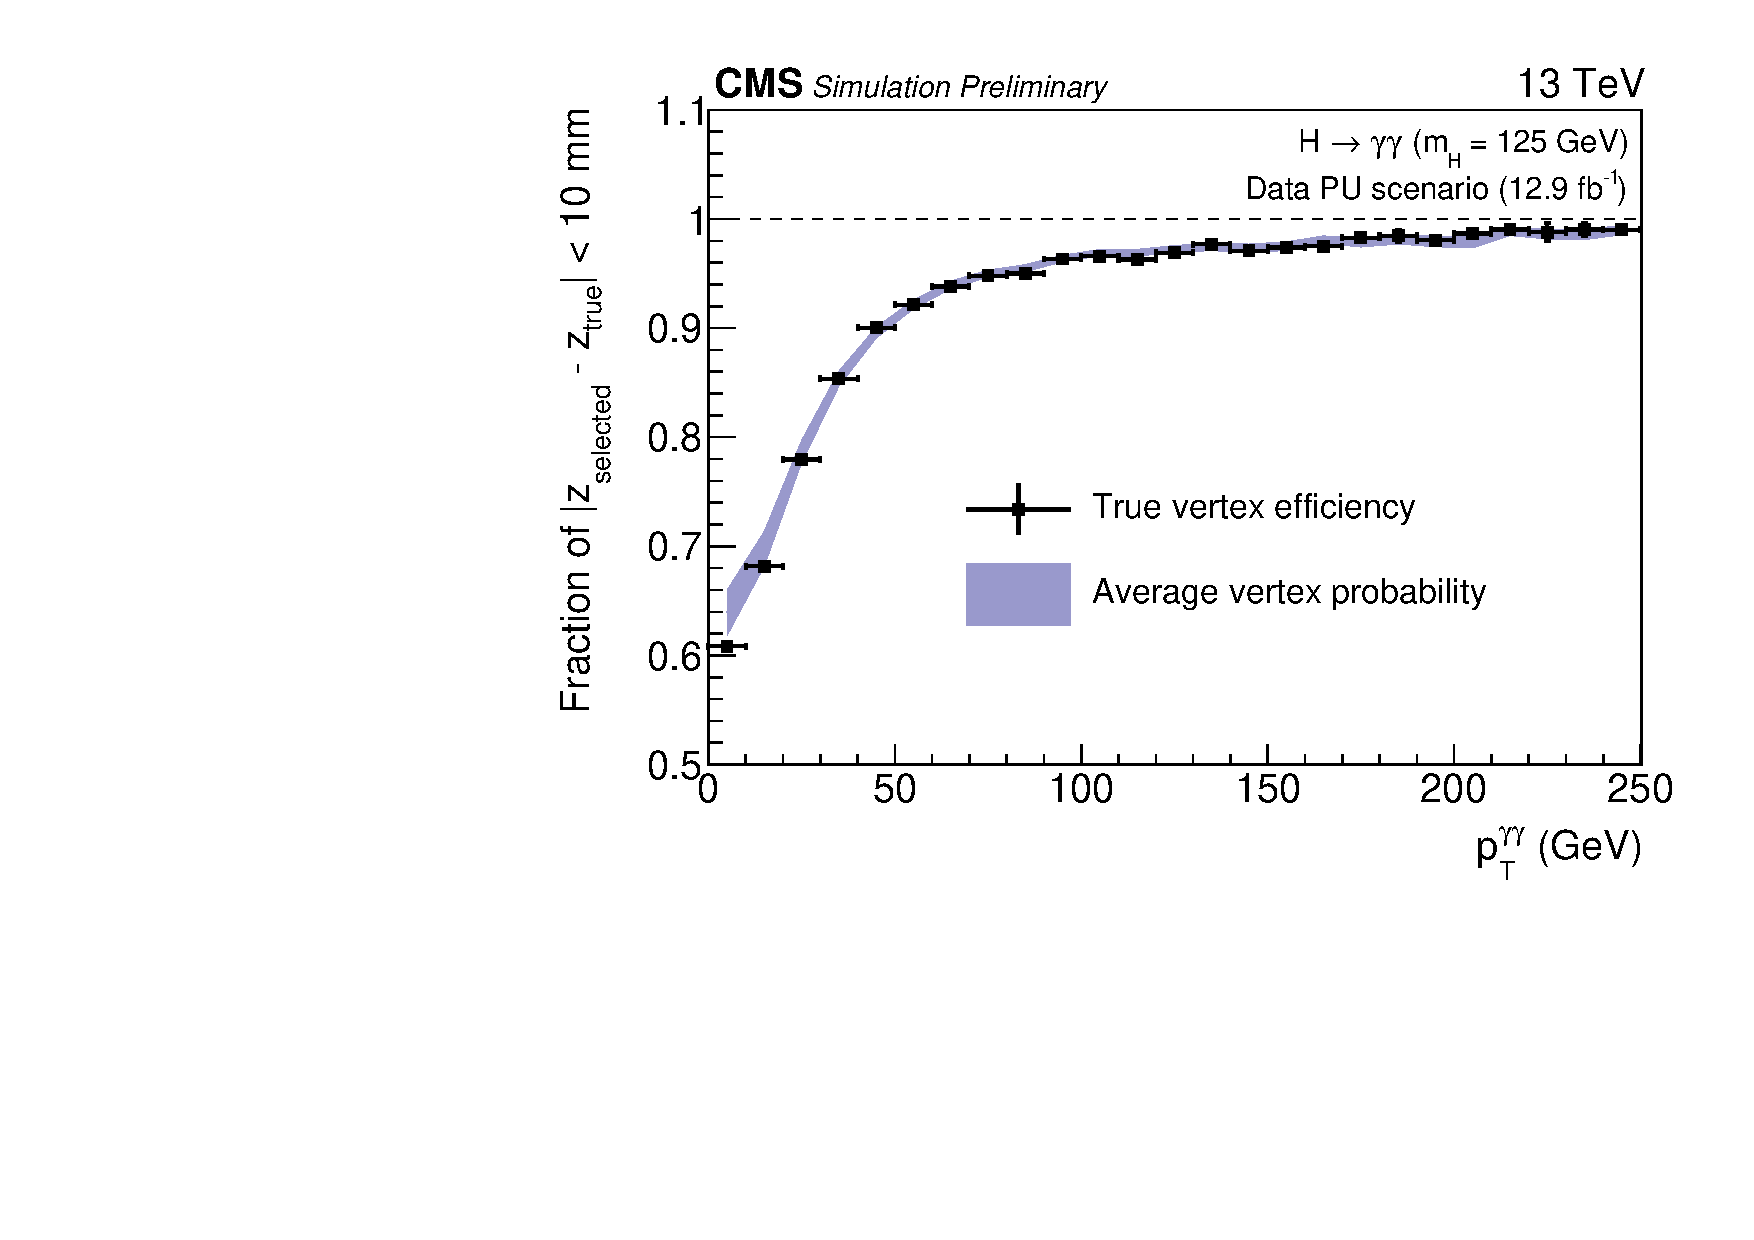
\includegraphics[width=0.45\textwidth]{recoFigures/Pt2016PU125BSReweighted12.pdf}
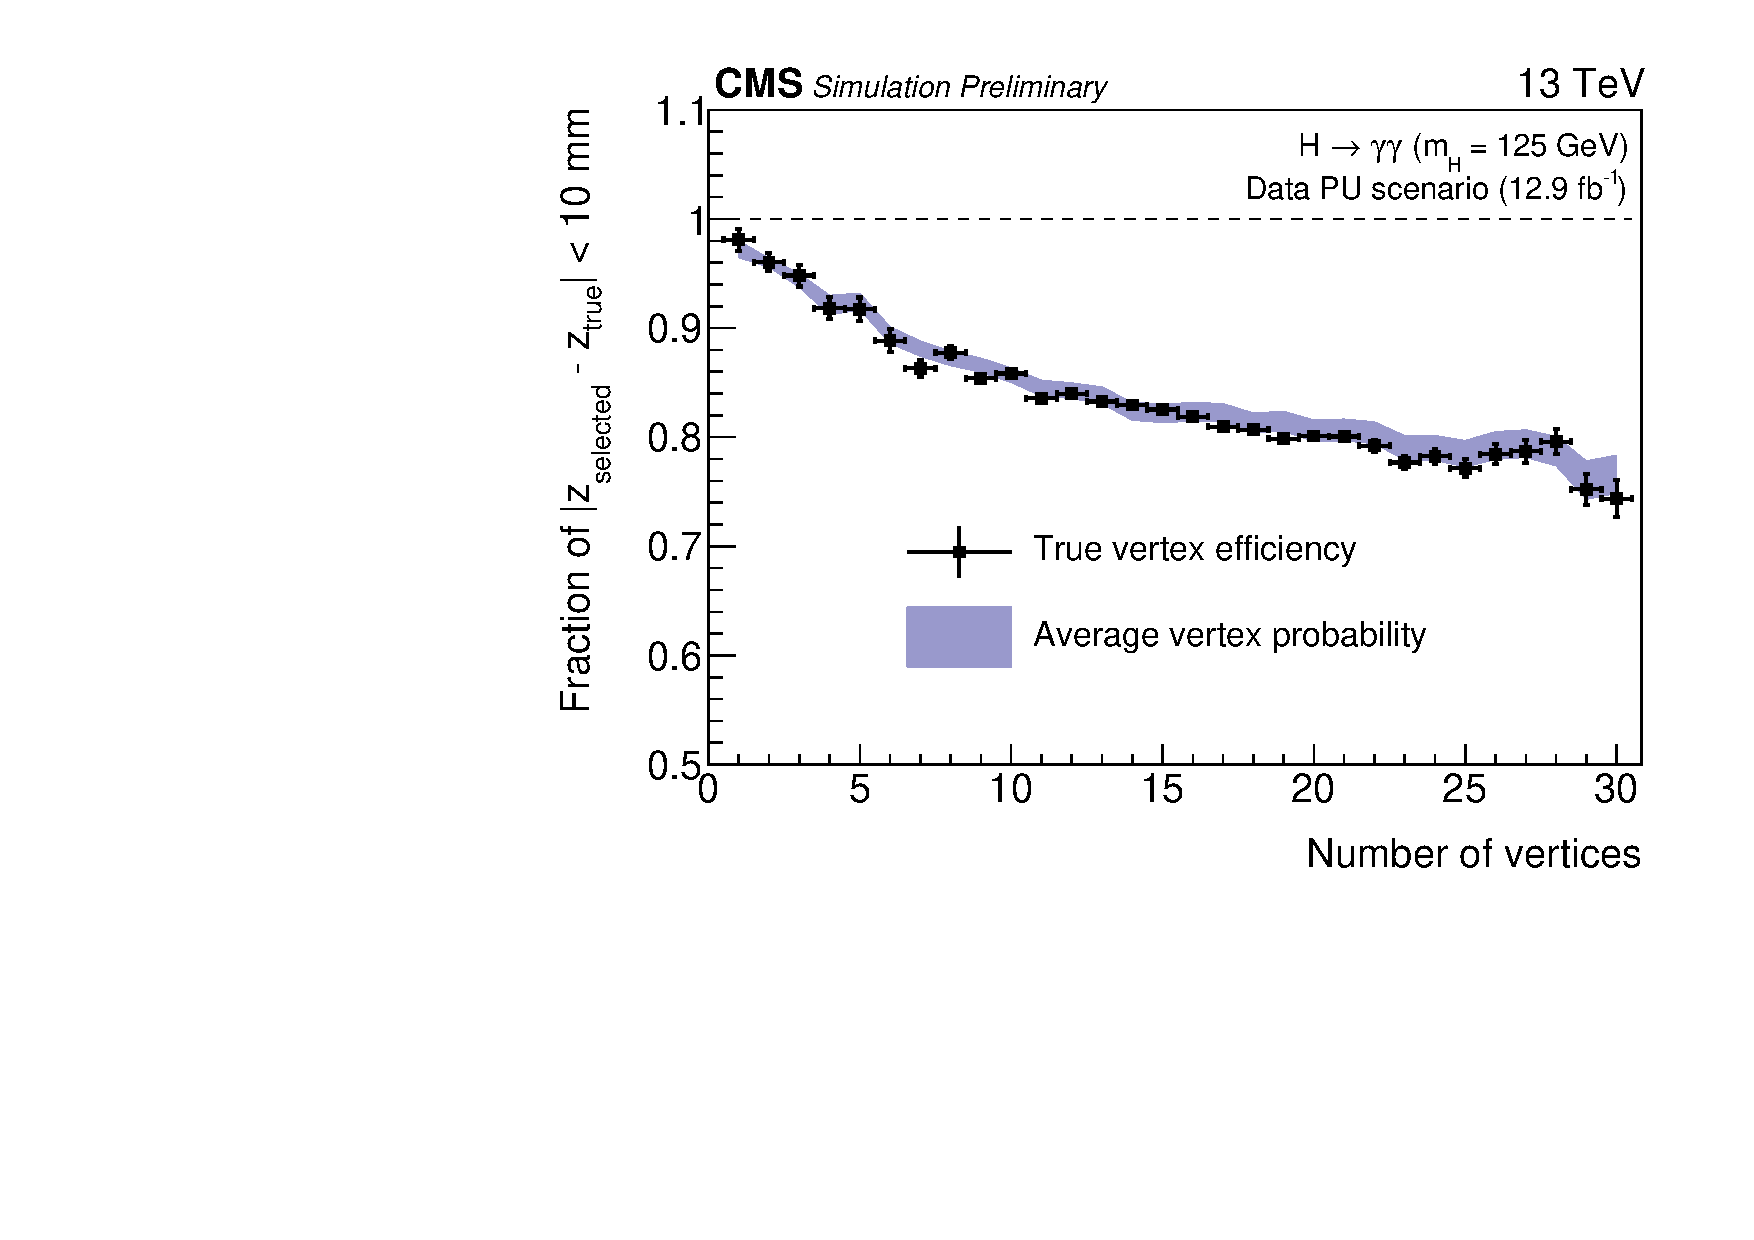
\includegraphics[width=0.45\textwidth]{recoFigures/Nvtx2016PU125BSReweighted12.pdf}
\caption{The efficiency to select a vertex within 1\cm of the true vertex in simulated \Hgg events as a function \pT and the number of vertices in the event. The estimated probability that the vertex was chosen within 1\cm is super-imposed. The uncertainty on the vertex-finding probability was determined using \Zmumu events. The simulation was re-weighted such that the distribution if the number of vertices and the width of the interaction region matched in data and simulation. }
\label{fig:reco:vtxidbdt_eff}
\end{figure}

\subsection{Correct Vertex Probability}

In cases where the chosen vertex is chosen the be over 1\cm away from the true one, the invariant mass resolution is dominated by the uncertainty on the vertex position, which can be large, significantly degrading the sensitivity of the analysis. It is therefore desirable to have a per-event estimate of how likely it is that the vertex was chosen within 1\cm of the true one. This information is then used to categorise events by sensitivity, as described in \Sec~\ref{}.

The estimate of the per-event vertex probability is obtained using a \BDT, which is labelled \VtxProbBdt. The input variables for this \BDT are:

\begin{itemize}
\item the number of reconstructed vertices in the event,
\item the \pT of the diphoton system,
\item the output scores of the three vertices ranked highest by the \VtxIdBdt,
\item the distance in the $z$-direction between the first- and second-highest ranked vertices,
\item the distance in the $z$-direction between the first- and third-highest ranked vertices,
\item the number of vertices in the three highest-ranked which used converted photon information.
\end{itemize}

The probability that the selected vertex is within 1\cm of the true vertex is estimated by parametrized as a function of the \VtxProbBdt output score using a $4^{th}$ order polynomial.This is done separately for converted and unconverted photons. The estimated vertex identification probability is shown alongside the vertex efficiency measured in simulation of \Fig~\ref{fig:reco:vtxidbdt_eff}. As for the \VtxIdBdt, the \VtxProbBdt was validated using \Zmumu events. 

\section{Other objects} 
\label{reco:sec:other}
\subsection{Jets}
\subsection{Electrons}
\subsection{Muons}
\subsection{Missing energy}
\subsection{Top quarks}

Lorem Ipsum \cite{PDGBooklet}.
